
% ===========================
\chapter{Grundlagen}
\label{grundlagen}
% ===========================

In diesem Kapitel werden die zum Verständnis nötigen Grundlagen für diese Arbeit erklärt. Dabei wird im Abschnitt \ref{grundlagen_fahren} der Stand der Technik von automatisierten Fahrfunktionen und deren Entwicklung beschrieben. Im Abschnitt \ref{grundlagen_nn} wird maschinelles Lernen im Allgemeinen und im Speziellen künstliche neuronale Netze, die für die Umsetzung dieser Arbeit nötig sind, beschrieben.


% ===========================
\section{Hochautomatisiertes Fahren}
\label{grundlagen_fahren}
% ===========================

Hochautomatisiertes Fahren wird in den vergangenen Jahren zunehmend von der Automobilindustrie vorangetrieben. Aktuelle \gls{fas} wie der Spurhalteassistant oder die Abstandsregelung sind nach der Norm SAE J3016 (Abbildung \ref{fig_level_autonomes_fahren}) bei Level 2 des autonomen Fahrens eingeordnet. Mit neuen Technologien werden immer mehr Funktionen für automatisiertes Fahren entwickelt und verknüpft. Es entstehen zunehmend komplexe Fahrfunktionen mit einer steigenden Anzahl möglicher Fahrsituationen und Szenarien \cite{king2017identification}. Das stellt Automobilhersteller und Automobilzulieferer vor eine große Herausforderung, da die Systemkomplexität wächst. Das schließt sowohl die Entwicklung von \gls{fas} als auch die dazu benötigten Testszenarien ein \cite{pfeffer2016continuous}.

In den folgenden Abschnitten wird erläutert wie aktuell diesen Herausforderungen begegnet wird. In Abschnitt \ref{grundlagen_fahren_entwicklung} wird ein allgemeiner Überblick über die aktuellen Entwicklungsmethodiken für \gls{fas} gegeben. Dabei wird besonders auf das Konzept \gls{vil} eingegangen. Danach werden in Abschnitt \ref{grundlagen_fahren_szenarien} bisherige Ansätze für die Klassifizierung von Fahrszenarien vorgestellt.

\begin{figure}[h]
\centering
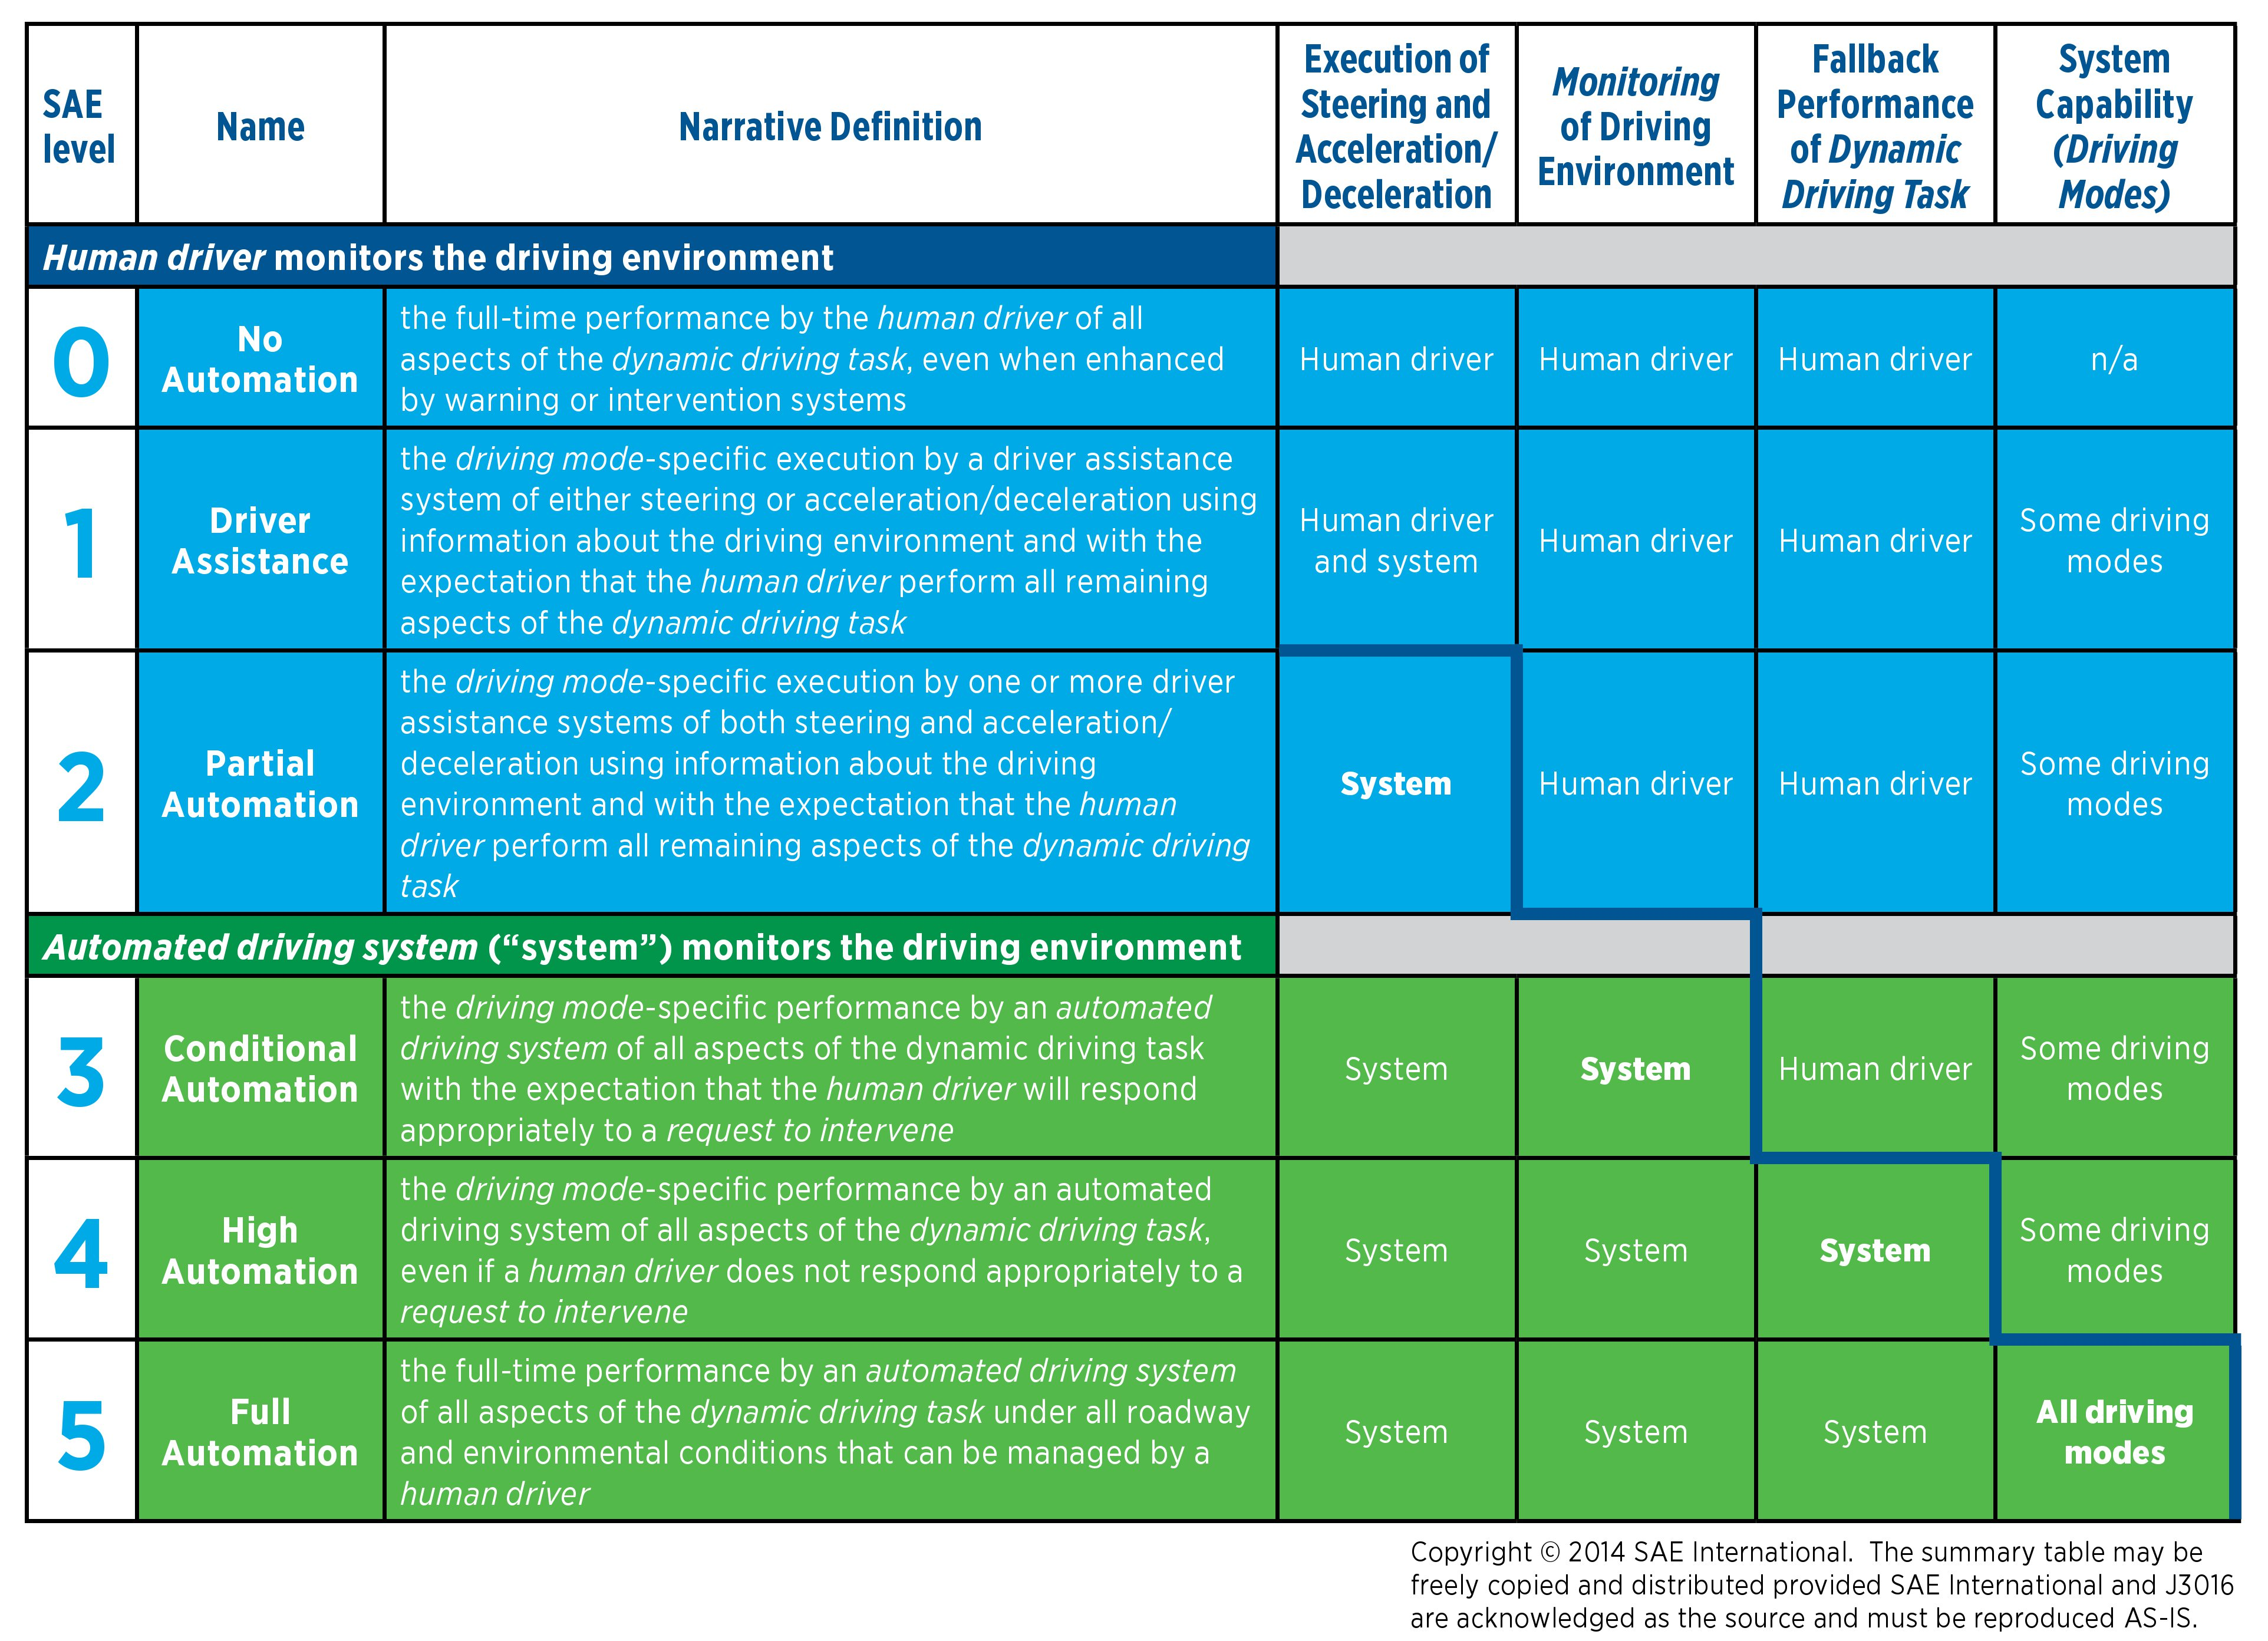
\includegraphics[scale=0.7]{level_autonomes_fahren.jpg}
\caption{Norm SAE J3016 für die Level des autonomen Fahrens, entnommen aus \cite{sae2014taxonomy}}
\label{fig_level_autonomes_fahren}
\end{figure}


% ===========================
\subsection{Entwicklung von Fahrerassistenzfunktionen}
\label{grundlagen_fahren_entwicklung}
% ===========================

\gls{fas} sind Funktionen im Kraftfahrzeug, die den Fahrer unterstützen. Diese Systeme nutzen Sensordaten, wie Radar-, Ultraschall-, oder Kameradaten, aus dem Fahrzeug um den Fahrer dann auf Basis der abgeleiteten Informationen zu unterstützen. Beispielsweise erkennt ein Spurhalteassistent wenn das Fahrzeug die Spur verlässt und kann die Fahrlinie korrigieren. 

\gls{fas} werden in der Automobilindustrie mit dem V-Modell entwickelt. Das V-Modell ist ein chronologischer Entwicklungsprozess und aus der Softwareentwicklung adaptiert \cite{vmodell2005}. Das V-Modell kann in einen linken absteigenden und einen rechten aufsteigenden Ast unterteilt werden. Der linke Ast enthält die Funktionsanforderungen, die nach unten weiter detailliert und aufgeschlüsselt werden. Der rechte Ast umfasst aufsteigend Funktionstests auf dem jeweiligen Detaillierungsgrad \cite{hakuli2015virtuelle}. Das V-Modell ist schematisch in Abbildung \ref{fig_v_modell} dargestellt.

\begin{figure}[h]
\centering
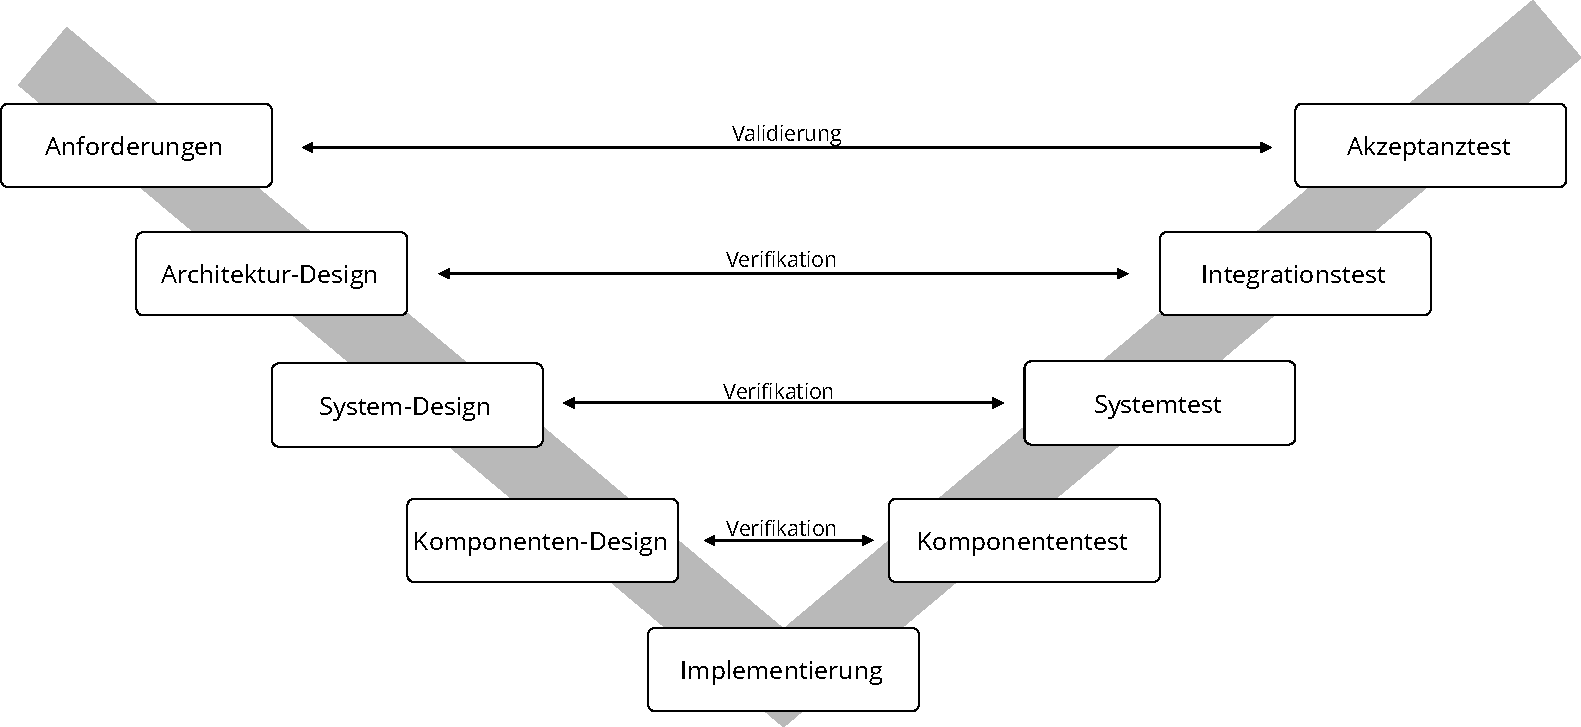
\includegraphics[scale=0.5]{v_modell.pdf}
\caption{V-Modell, adaptiert von \cite{hakuli2015virtuelle}}
\label{fig_v_modell}
\end{figure}

Die Schritte auf dem absteigenden und aufsteigenden Ast haben jeweils eine Beziehung. Jeder Test auf dem aufsteigenden Ast verifiziert bzw. validiert den dazugehörigen Entwicklungsschritt auf dem absteigenden Ast. Demenstsprechend werden oben im V-Modell die Kundenanforderungen auf dem absteigenden Ast erfasst und auf dem aufsteigenden Ast validiert. Unten im V-Modell werden einzelne Hardware- oder Softwarekomponenten entwickelt, die die entsprechenden Kundenanforderungen von oben lösen sollen, und auf dem aufsteigenden Ast verifiziert \cite{hakuli2015virtuelle}.

Die Validierung und Verifikation von \gls{fas} folgt dem Testkonzept. Ein Testkonzept umfasst die Analyse des Testobjektes, die Generierung von Testfällen, die Durchführung von Tests und schließlich die Testauswertung \cite{schuldt2013effiziente}.

\begin{figure}[h]
\centering
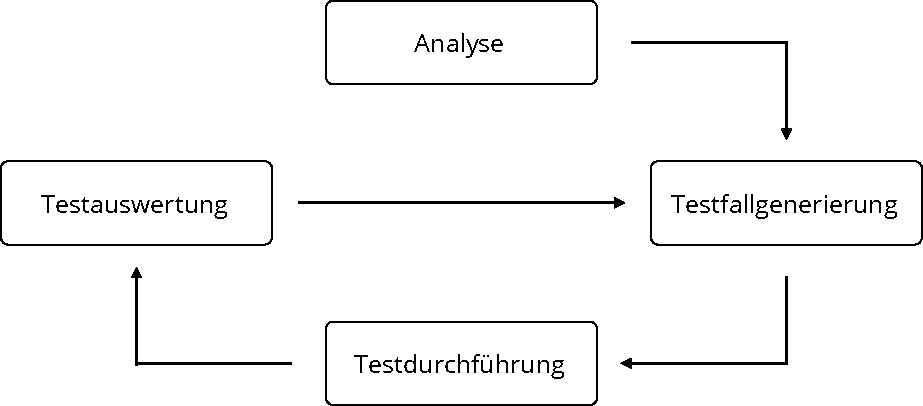
\includegraphics[scale=0.5]{testfallerstellung.pdf}
\caption{Testfallerstellung, von \cite{schuldt2013effiziente}}
\label{fig_testfallerstellung}
\end{figure}

Testfälle werden bereits möglichst früh im Entwicklungsprozess erstellt um die Qualität von \gls{fas} und einzelnen Komponenten möglichst hoch zu halten \cite{wachenfeld2015freigabe}. Hierfür werden in der Praxis virtuelle Fahrversuche eingesetzt. Die Idee ist eine stufenweise Digitalisierung von Komponenten aus dem realen Fahrversuch mit den Zielen die Reproduzierbarkeit zu steigern, den Aufwand zu reduzieren und insgesamt flexibler zu werden. Im virtuellen Fahrversuch werden in der frühen Konzeptphase alle Komponenten virtuell getestet und dann schrittweise durch Hardwarekomponenten ersetzt. Schließlich werden alle Komponenten im realen Fahrversuch auf der Straße mit realem Fahrer und anderen Verkehrsteilnehmern getestet \cite{hakuli2015virtuelle}. In diesem Zusammenhang spielen die Konzepte \gls{mil}, \gls{sil}, \gls{hil} und \gls{vil} eine wichtige Rolle. Mit \gls{mil} und \gls{sil} werden Funktionen auf Basis von Simulationsmodellen getestet. Dabei werden Hardwarekomponenten simuliert. Mit fortschreitender Entwicklung werden immer mehr Simulationskomponenten durch die entsprechende Hardware ersetzt und mit \gls{hil} und \gls{vil} werden diese getestet \cite{hakuli2015virtuelle}.

---

Mit steigender Komplexität in der Entwicklung, bedingt durch hochautomatisierte Funktionen, werden für die Validierung und Verifikation von \gls{fas} neue Testmethoden benötigt \cite{bach2017reactive}. Besonders \gls{fas} die kritische Situationen unterstützen, wie zum Beispiel eine automatische Notbremsung, können nicht mehr mit lange etablierten Methoden getestet werden \cite{bock2008vehicle}. 







Nach den Grundsätzen des Projektmanagements erfolgt die Freigabe erst dann, wenn die zuvor definierten Anforderungen von diesem technischen System erfüllt werden. Diese Anforderungen haben unterschiedlichste Ursprünge, wie beispielsweise Kunden, Normen oder Gesetze. Verschiedene Bereiche werden durch die Anforderungen adressiert: Darunter fallen nicht zuletzt aus Gründen der Typgenehmigung1 als auch der Produkthaftung2 Anforderungen an die Sicherheit des technischen Systems. \cite{wachenfeld2015freigabe}


-----------------------------------


\cite{berg2015vehicle}:
Für die effiziente und kostengünstige Entwicklung sowie Absicherung hat sich, über die Entwicklung von realen Funktionen im Fahrzeug hinaus, ein zweiter Entwicklungsast mit einer vir- tuellen Entwicklung etabliert. So werden bereits in einer frühen Phase neue Algorithmen mithilfe von Software-in-the-Loop prototypisch entwickelt und getestet (vgl. ▶ Kap. 8) oder neue Sensoren sowie Aktoren mithilfe von Hardware-in-the-Loop-Test- ständen evaluiert, ohne dass hierfür ein Fahrzeug aufgebaut werden muss. Gleichzeitig erfolgt mit- hilfe von Fahrsimulatoren (Driver-in-the-Loop, vgl. ▶ Kap. 9) eine Überprüfung des Fahrerverhaltens sowie der Beherrschbarkeit.

Das Vehicle in the Loop (VIL) schließt die Lü- cke zwischen Fahrsimulation und Realversuchen.


-- Einsatz MiL, SiL, HiL
Um die funktionale Sicherheit neuer Fah- rerassistenzsysteme (FAS) abzusichern, kommen bei OEMs und Zulieferern je nach Entwicklungsphase unterschiedliche Test- und Bewertungsverfahren zum Ein- satz. Simulationsmethoden wie Model-in- the-Loop (MiL) und Software-in-the-Loop (SiL) werden vor allem in einer frühen, Hardware-in-the-Loop (HiL) in einer spä- teren Entwicklungsphase eingesetzt. \cite{schwab2014durchgangige}

-- Aufwand test FAS
Die Systeme werden in ein virtuelles Fahr- zeug integriert und im virtuellen Fahrver- such geprüft. Auf diese Weise können in sehr kurzer Zeit zahlreiche Tests unter beliebig konfigurierbaren und reprodu- zierbaren Bedingungen durchgeführt werden [1]. Diese simulativen Methoden sind allerdings kein Ersatz für den realen Fahrversuch. Auch wenn die aktuellen Modelle sehr gut sind, besteht die Unsi- cherheit, dass die Ergebnisse nicht exakt auf das reale Fahrzeugverhalten übertrag- bar sind. Darüber hinaus ist eine subjek- tive Bewertung im Fahrversuch unerläss- lich, um die Akzeptanz des Fahrers zu gewährleisten. Das Testen von FAS im klassischen Fahrversuch auf Straßen wird jedoch mit zunehmender Komplexität der Systeme immer aufwendiger. Während bei Ein- parkassistenten hauptsächlich nur ste- hende Objekte variiert werden müssen, um verschiedene Parkszenarien darzu- stellen, wird bei Systemen zur Unfall- vermeidung wie dem Notbremsassisten- ten mindestens ein potenzieller Unfall- gegner benötigt. In derzeit eingesetzten Verfahren werden hierfür sogenannte Dummy-Targets eingesetzt (zum Beispiel in [2]). Diese Ziele sind hauptsächlich für Auffahrszenarien im Längsverkehr aus- gelegt. Weitere relevante Verkehrssitua- tionen, wie etwa Querverkehr an einer Kreuzung, plötzlich einscherende Fahr- zeuge oder die Kollisionsgefahr mit Fußgängern oder Radfahrern können nur eingeschränkt beziehungsweise mit erheblichem Aufwand untersucht werden. \cite{schwab2014durchgangige}

-- ViL als Lösung mit vielen Vorteilen
Die neue Vehicle-in-the-Loop-Simulation (ViL) ist nach HiL und SiL eine innovative Methode, um die Komplexität bei der funktionalen Absicherung von Fahrerassistenzsystemen beherrschbar zu machen und gleichzeitig den Testaufwand zu reduzieren. Diese Methode kombiniert die Vorteile des Fahrversuchs und der Simulation, indem ein reales Fahrzeug in eine virtuelle Verkehrsumgebung eingebunden wird. \cite{schwab2014durchgangige}

Dieses Testkonzept bietet folgende Vorteile:
: reale Fahrdynamik
: weniger materieller Aufwand als im rein realen Fahrversuch
: reproduzierbare Testbedingungen
: beliebig konfigurierbare Szenarien. 

Weitere Anwendungsfelder für ViL sind unter anderem das Testen von Spur- wechselassistenten, Notbremsassistenten mit und ohne Fußgänger- beziehungs- weise Radfahrererkennung, Ausweich- assistenten sowie die Untersuchung kom- plexer, autonomer Fahrfunktionen im virtuell fließenden Verkehr. \cite{schwab2014durchgangige}





-- XiL
While real world validation is indispensable, it hampers reproducibil- ity. The preliminary development phase is characterized by tight re- sources, frequent changes in design and an iterative modus operandi. Scant experience with the system properties leads to regular realign- ments and refactorings. To achieve satisfying results within an appro- priate time span, besides the RP approach further stimuli for iterative test of control systems are required. These range from test vectors modelling certain interesting waveforms and replay of recorded data to more sophisticated approaches such as Time Partition Testing (TPT) [2], which facilitates systematic testing of embedded systems with continuous behavior, or X-in-the-loop (XiL) simulation [3-5]. XiL represents a simulation based methodology for the test of embed- ded systems over all development stages of the automotive industry. The selection of the appropriate stimuli depends on the specific char- acteristics of the System under Test (SuT). As shown in Figure 1, closed-loop control systems require stimulation by methods such as XiL, RP or TPT, which offer a sufficient degree of reactiveness. Un- fortunately, these elaborate methods require significant resources for deployment and maintenance. \cite{bach2017reactive}



-- Innovative Funktionen nicht losgelöst von Umwelt
Insbesondere die Fahrzeugentwicklung ist von vielen Innovatio- nen geprägt, die den Komfort, die Effizienz sowie die Sicherheit verbessern und optimieren sollen. Um ein globales Optimum zu erreichen, darf das System Fahrzeug nicht losgelöst von den Sys- temen Umwelt und Fahrer betrachtet werden. \cite{albers2010x}

-- für C2X gibt es nur beschränkt testmöglichkeiten
Car-to-X-(beziehungsweise Car2X)-Technologien sorgen für die notwendige Vernetzung. Reale Fahrversuche sind aber mit einem enormen Kosten- und Zeitaufwand verbunden. Um diese durch- zuführen und Szenarien abzubilden, müssen geeignete Testgelän- de sowie eine ausreichende Anzahl an Fahrzeugen mit prototypi- schen Car2X-Systemen vorhanden sein. Zudem bieten Tests in der realen Welt oft ein geringes Maß an Reproduzierbarkeit [2]. Ak- tuell beschränken sich Simulationen im Bereich Car2X auf Appli- kations- und Protokolltests [2].\cite{albers2010x}


% ===========================
\subsection{Klassifizierung von Fahrszenarien}
\label{grundlagen_fahren_szenarien}
% ===========================

- Terminologie, Unterschiedung Szene, Szenario, ...
- Tabelle + Erklärung

Duis autem vel eum iriure dolor in hendrerit in vulputate velit esse molestie consequat, vel illum dolore eu feugiat nulla facilisis at vero eros et accumsan et iusto odio dignissim qui blandit praesent luptatum zzril delenit augue duis dolore te feugait nulla facilisi.   


% ===========================
\section{Künstliche Neuronale Netze}
\label{grundlagen_nn}
% ===========================

Duis autem vel eum iriure dolor in hendrerit in vulputate velit esse molestie consequat, vel illum dolore eu feugiat nulla facilisis.


% ===========================
\subsection{Maschinelles Lernen}
\label{grundlagen_nn_ml}
% ===========================

Duis autem vel eum iriure dolor in hendrerit in vulputate velit esse molestie consequat, vel illum dolore eu feugiat nulla facilisis at vero eros et accumsan et iusto odio dignissim qui blandit praesent luptatum zzril delenit augue duis dolore te feugait nulla facilisi. 


% ===========================
\subsection{Convolutional Neural Network}
\label{grundlagen_nn_cnn}
% ===========================


\begin{table}[h]
\centering
\begin{tabular}{l | l | l}
A & B & C \\
\hline
1 & 2 & 3 \\
4 & 5 & 6
\end{tabular}
\caption{very basic table}
\label{tab:abc}
\end{table}


% ===========================
\subsection{Recurrent Neural Network}
\label{grundlagen_nn_rnn}
% ===========================

Lorem ipsum dolor sit amet, consectetuer adipiscing elit, sed diam nonummy nibh euismod tincidunt ut laoreet dolore magna aliquam erat volutpat \cite{latexcompanion}. 


% ===========================
\subsection{Training mit synthetischen Daten}
\label{grundlagen_nn_synthetisch}
% ===========================

Lorem ipsum dolor sit amet, consectetuer adipiscing elit, sed diam nonummy nibh euismod tincidunt ut laoreet dolore magna aliquam erat volutpat \cite{latexcompanion}. 


